\section{Wireframe (Low-Fidelity)}

Setelah kebutuhan diidentifikasi dan persona dibuat, langkah selanjutnya adalah memvisualisasikan solusi melalui \textbf{wireframe}---sketsa kasar (\textit{low-fidelity}) yang menunjukkan struktur dan tata letak halaman tanpa detail visual. Wireframe fokus pada \textbf{apa} yang ada di halaman dan \textbf{di mana} letaknya---bukan pada bagaimana tampilannya. Membangun wireframe terlebih dahulu jauh lebih murah dan cepat daripada langsung coding atau mockup---perubahan pada kertas atau Figma membutuhkan menit, sedangkan perubahan pada kode bisa membutuhkan hari \cite{mdnLearn}.

Wireframe biasanya dibuat dalam warna abu-abu atau hitam-putih, tanpa gambar sesungguhnya, dan menggunakan placeholder untuk teks dan gambar. Alat yang umum digunakan untuk membuat wireframe antara lain kertas dan pensil, Balsamiq, Whimsical, atau Figma dalam mode wireframe \cite{webdevLearn}.

Manfaat wireframe antara lain: (1) cepat dibuat dan mudah diubah; (2) membantu tim mendiskusikan struktur tanpa terdistraksi oleh detail visual; (3) dapat diuji dengan pengguna sejak dini (\textit{paper prototyping}); dan (4) menjadi dasar untuk membuat mockup yang lebih detail (Bab 4).

\subsection{Langkah Membuat Wireframe}

Proses pembuatan wireframe mengikuti langkah-langkah berikut: (1) tentukan halaman apa saja yang perlu di-wireframe berdasarkan user flow; (2) identifikasi elemen utama setiap halaman (header, navigasi, konten utama, sidebar, footer); (3) gambar tata letak menggunakan kotak dan garis; (4) tambahkan placeholder teks dan gambar; dan (5) review bersama tim dan pengguna lalu iterasi.

\begin{figure}[htbp]
\centering
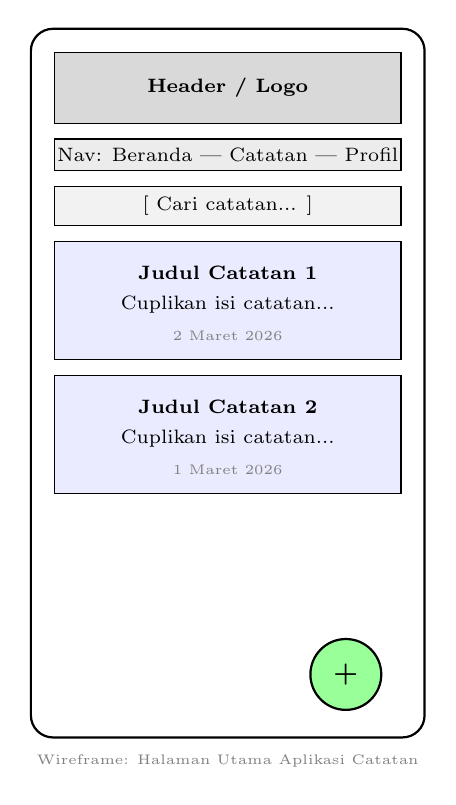
\begin{tikzpicture}[transform shape, every node/.style={font=\scriptsize}]
  % Phone frame
  \draw[thick, rounded corners=8pt] (0,0) rectangle (5,9);
  
  % Header
  \draw[fill=gray!30] (0.3,7.8) rectangle (4.7,8.7);
  \node[font=\scriptsize\bfseries] at (2.5,8.25) {Header / Logo};
  
  % Navigation
  \draw[fill=gray!15] (0.3,7.2) rectangle (4.7,7.6);
  \node at (2.5,7.4) {Nav: Beranda | Catatan | Profil};
  
  % Search bar
  \draw[fill=gray!10] (0.3,6.5) rectangle (4.7,7.0);
  \node at (2.5,6.75) {[ Cari catatan... ]};
  
  % Card 1
  \draw[fill=blue!8] (0.3,4.8) rectangle (4.7,6.3);
  \node[font=\scriptsize\bfseries] at (2.5,5.9) {Judul Catatan 1};
  \node at (2.5,5.5) {Cuplikan isi catatan...};
  \node[font=\tiny, gray] at (2.5,5.1) {2 Maret 2026};
  
  % Card 2
  \draw[fill=blue!8] (0.3,3.1) rectangle (4.7,4.6);
  \node[font=\scriptsize\bfseries] at (2.5,4.2) {Judul Catatan 2};
  \node at (2.5,3.8) {Cuplikan isi catatan...};
  \node[font=\tiny, gray] at (2.5,3.4) {1 Maret 2026};
  
  % FAB button
  \draw[fill=green!40, thick] (4.0,0.8) circle (0.45);
  \node[font=\bfseries] at (4.0,0.8) {+};
  
  % Label
  \node[font=\tiny, gray] at (2.5, -0.3) {Wireframe: Halaman Utama Aplikasi Catatan};
\end{tikzpicture}
\caption{Contoh wireframe halaman utama aplikasi catatan harian (low-fidelity)}
\end{figure}

Setelah wireframe divalidasi bersama tim dan pengguna, langkah selanjutnya adalah mengembangkannya menjadi \textbf{mockup} (high-fidelity) dan \textbf{prototipe} interaktif. Pembahasan mockup, prinsip desain visual, aksesibilitas, dan UX dilanjutkan di Bab 4.
